\maketitle

\section*{Introduction}
For this week, to review some review papers I chose classification of motor imagery as the topic for research. Motor imagery refers to the voluntary imagination of performing a certain physical action without physically doing it. For example, mentally executing moving right arm, left foot etc. but not actually moving the right arm or left foot. Data associated with those mental execution is collected via EEG, MEG, fNIRS etc. and classification of these data into different activity class is a significant part of Brain-Computer Interface (BCI) research that impacts rehabilitation of disabled person. 

Starting from data acquisition, preprocessing, to feature extraction and classification- the different stages in Motor Imagery based Brain-Copmputer Interface (MI-BCI) have been focused on for research and improvement. For these review papers, I judged them based on how they approached the review and if it was thorough enough within their point of view. Except for 1 or 2, I found majority of the survey papers to be consistent and not much lacking based on my own knowledge of the area.\\

\subsection*{A Review on the Components of EEG-based Motor Imagery Classification with Quantitative Comparison}\cite{rahman_review_2017}

My main critique of this paper is that it had a good plan, but it was not executed well. This is what I would say is a flawed survey paper. With some more time and effort, it could have been a better paper that could achieve everything it set out to. The paper is meant to provide a review of methods used in different steps of MI-BCI as well as analyze it so it could act as a reference to check the performance of those methods. However, the authors only used one set of data which is not enough for a quantitative analysis and categorically judging a method's performance. Also, the methods were not comprehensive enough, adding more to the reason why the paper may not have been cited much. 
\\The way some sections were explained is not consistent. For example,  mathematical equations and notations for some methods were given but not for others. Literature review of these concepts were not thorough enough, with only a few papers mentioned for each tools.
The work in this paper would have been better if they picked one or two stages in MI-BCI workflow and carried out a thorough analysis of them like \cite{aggarwal_signal_2019} or \cite{thomas_analysis_2013} did. In \cite{thomas_analysis_2013}, the authors only focused on the performance evaluation metrics for different types of MI-BCI, whereas \cite{aggarwal_signal_2019} focuses on only the signal processing techniques. To take things further, the authors could have also tried to justify why certain results could have tried to justify why the results are how they are. \\

\subsection*{Deep learning for motor imagery EEG-based classification: A review}\cite{al-saegh_deep_2021}
This is a paper that has a specific theme which is deep learning and the authors adhered to that theme throughout the paper. However, they could have talked about the approaches more critically since deep learning with BCI is a fairly new field which still has a lot of significant issues to work through. One big issue is there is not enough BCI data available for a strong, generalizable deep learning model. Often times, data augmentation is considered as a solution but it is not as straightforward with neural signal as it is with, for example, image data. 
In contrast, \cite{khademi_review_2023} compared deep learning approaches to conventional methods in MI-BCI. 
\\The table in the appendix summarizing their findings is a useful addition that helps their objective of serving as a guide for finding appropriate neural network structure and hyperparameter for new BCI researches. \\

\subsection*{Deep learning tech-
niques for classification of electroencephalogram (EEG) motor imagery
(MI) signals: a review}\cite{altaheri_deep_2023}
Another very recent review paper that also looks at deep learning in MI-BCI is \cite{altaheri_deep_2023}. The authors clearly stated the criteria and how they proceeded with it- criteria for finding papers, and evaluation.
Aside from the paper being very well structured, it also talks about different approaches to deep learning and not just the architecture of the network, which I thought was missing from \cite{al-saegh_deep_2021}. For example, representative, generative and hybrid deep learning models. Unlike the previous paper \cite{al-saegh_deep_2021}, this paper contains a significant section addressing some vital questions about deep learning in MI-BCI. Some thing I noticed this paper missed is graph neural network or graph based deep learning approaches. Although a quick scholar search showed there was no or barely any research with GNN on MI during the time period this paper focused on (2011-2020). So, this could be a "gap"/ future review paper idea, to survey Graph based approached in all BCI research, as it might be too little for only MI-BCI. 

\subsection*{EEG-Based
Brain-Computer Interfaces Using Motor-Imagery: Techniques and Challenges}\cite{padfield_eeg-based_2019}
From my search, the most cited paper was this \cite{padfield_eeg-based_2019}. Main theme I noticed with this paper that was missing from the others was that it talks about every method from a critical point of view, that is, talking about not only their uses but also where each of them has issues or shortcomings. The authors also pointed out different areas for MI-BCI use and provided body of previous works for each areas. The paper also includes sections on challenges with commercialization of BCI which is something I have not noticed in the other review papers described here. 

\subsection*{Review of Critical Challenges in MI-BCI: From conventional to deep learning methods}\cite{khademi_review_2023}
For review of deep learning methods in MI-BCI, \cite{khademi_review_2023} brought something interesting to the table by comparing traditional methods with deep learning methods. This paper is written for someone who is already familiar with the vernacular of BCI. Like most papers I found during this assignment, this paper focuses on methods that work with pre-recorded BCI data. Which leads me to believe that I found another "gap" and that is reviewing BCI systems that work with data collected online as they work.


The two gaps I found for future review are shown in red in the following image. 
\begin{figure}[h]
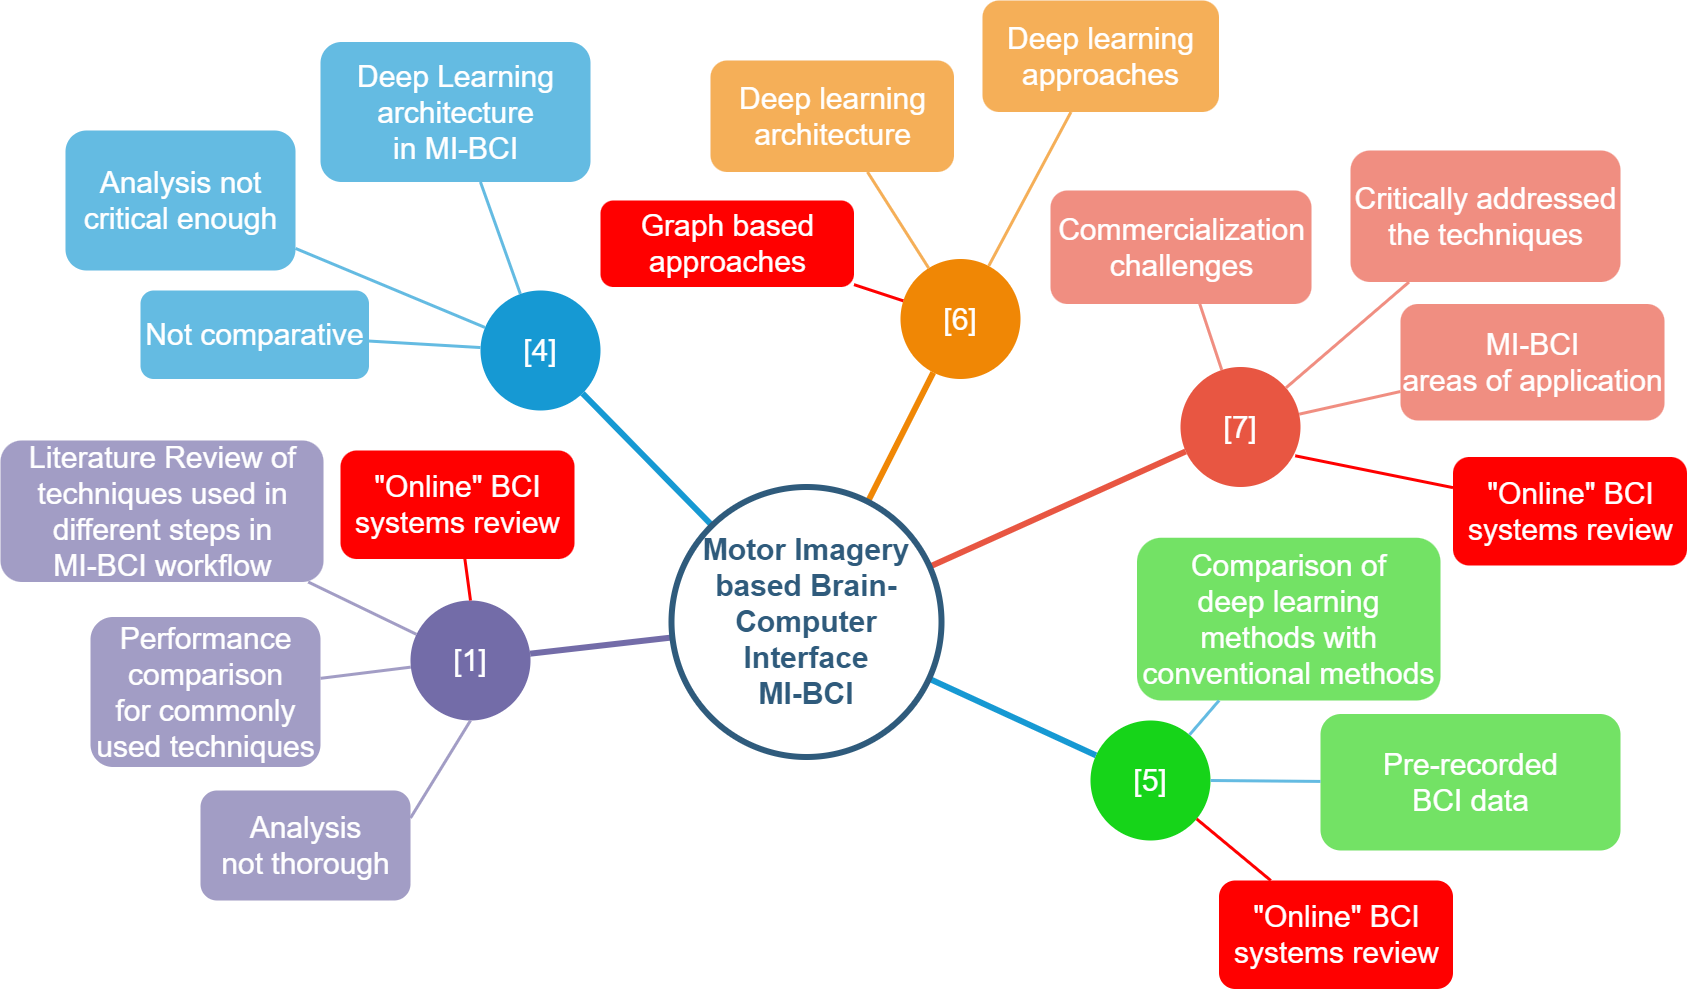
\includegraphics[width=1\textwidth, inner]{body/map}
\caption{Map}
\label{fig:figure2}
\end{figure}

\vspace{5mm}
Link to git repository containing this work: \url{https://github.com/r-nusrat/CS_6000_week3}
\nocite{*}